\documentclass[conference]{IEEEtran}
\IEEEoverridecommandlockouts
\usepackage{cite}
\usepackage{amsmath,amssymb,amsfonts}
\usepackage{graphicx}
\usepackage{textcomp}
\usepackage{xcolor}
\usepackage{booktabs}
\usepackage[T1]{fontenc}
\usepackage[utf8]{inputenc}
\usepackage{tikz}
\usetikzlibrary{positioning,calc,arrows.meta}
\usepackage{multirow}
\usepackage{array}
\usepackage{microtype}
\usepackage{float}
\emergencystretch=2em
\setlength{\intextsep}{4pt plus 2pt minus 2pt}
\setlength{\textfloatsep}{4pt plus 2pt minus 2pt}
\renewcommand{\floatpagefraction}{0.99}

\begin{document}

\title{Design and Evaluation of Information Retrieval Methods for Statement of Applicability Mapping of ISO/IEC 27001:2022 Annex A.5--A.8}

\author{
  \IEEEauthorblockN{\textsuperscript{1st}Muhammad Hilmi Dzaki Wismadi}
  \IEEEauthorblockA{\textit{Department of Electrical and Information Engineering}\\
    \textit{Universitas Gadjah Mada}\\
    Yogyakarta, Indonesia\\
    muhammadhilmidzakiwismadi@mail.ugm.ac.id}
  \and
  \IEEEauthorblockN{\textsuperscript{2nd}Dani Adhipta, S.Si., M.T.}
  \IEEEauthorblockA{\textit{Department of Electrical and Information Engineering}\\
    \textit{Universitas Gadjah Mada}\\
    Yogyakarta, Indonesia\\
    dani@ugm.ac.id}
}

\maketitle

\begin{abstract}
Compliance auditing against ISO/IEC 27001:2022 requires mapping organizational
policy documents to specific Annex~A controls, a process that is time-consuming
and error-prone when performed manually. This paper evaluates retrieval
strategies within a Retrieval-Augmented Generation (RAG) framework to support
automated Statement of Applicability (SoA) control mapping. Three design axes
are investigated: the weight composition between dense and sparse retrieval,
the candidate pool size for cross-encoder reranking, and the score fusion
weight between hybrid retrieval and cross-encoder scores. Experiments are
conducted using 77~queries derived from Directorate of Information Technology
(DTI) Universitas Gadjah Mada policy documents against a knowledge base of
93~ISO/IEC 27001:2022 Annex~A controls. Non-parametric statistical testing
confirms that all three design axes significantly affect retrieval performance.
A per-query analysis further reveals that hybrid retrieval and cross-encoder
reranking exhibit complementary strengths depending on query characteristics,
providing a basis for the optimal score fusion configuration identified in
this study.
\end{abstract}

\begin{IEEEkeywords}
ISO/IEC 27001, Statement of Applicability, hybrid retrieval, cross-encoder
reranking, retrieval-augmented generation, information security audit
\end{IEEEkeywords}

% ============================================================
\section{Introduction}
% ============================================================

The accelerating pace of digital transformation has expanded organizational
attack surfaces, making information security management increasingly complex.
The Check Point Global Cyber Attack Report~2026 indicates that the education
sector experienced an average of 4,749~cyber attacks per organization per
week, a 7\% year-over-year increase, with the Asia-Pacific region averaging
3,040~attacks per week~\cite{checkpoint2026}. In response, organizations
adopt ISO/IEC~27001, which provides a risk-based Information Security
Management System (ISMS) framework~\cite{calder2023iso27001,isoiec20227001}.
The 2022 revision consolidated Annex~A from 114 to 93~controls across four
categories: organizational, people, physical, and
technological~\cite{calder2023iso27001}.

However, ISO~27001 compliance auditing remains operationally burdensome.
Certification can span 6--12 months with significant cost~\cite{marques2024automating},
primarily due to analytical activities such as control-to-document mapping,
evidence evaluation, and Statement of Applicability (SoA) preparation.
The SoA, which links risk assessment outcomes to implemented controls, is
particularly critical: auditors must verify that each Annex~A control is
consistently evaluated with supporting evidence, a process prone to
inconsistency and scalability limitations when performed manually~\cite{csam2024}.

Retrieval-Augmented Generation (RAG) architectures offer a promising
approach for document-grounded analysis by combining natural language
understanding with external knowledge retrieval. Prior work demonstrates
that RAG performance is heavily influenced by retrieval quality, including
query representation, document search, and relevance
ranking~\cite{gupta2025compliance,lajbr2025,auditgpt2025,reguquery2025}.
In audit and compliance domains, Liu et~al.~\cite{lajbr2025} combined BM25
and dense retrieval with weighted Reciprocal Rank Fusion for audit-to-regulation
mapping. Gupta et~al.~\cite{gupta2025compliance} applied DPR with
cross-encoder reranking for GDPR/CCPA compliance checking. Ravishankar and
Varalakshmi~\cite{ravishankar2025hybrid} integrated hybrid retrieval,
reranking, and score fusion for financial document QA. Rustamov
et~al.~\cite{rustamov2025tax} compared sparse, dense, and reranking
strategies for tax law QA. Elkiran and Rasheed~\cite{elkiran2026empirical}
provided empirical evidence that retriever selection, similarity function,
and reranker choice significantly affect RAG performance.

Hybrid retrieval combines sparse methods (e.g., BM25) that capture exact
lexical matches with dense methods (e.g., neural embeddings) that capture
semantic similarity. This combination is particularly beneficial in
regulatory domains where both explicit terminology matching and contextual
understanding are required. Cross-encoder reranking further refines
candidate rankings by jointly encoding query--document pairs, achieving
higher precision at the cost of increased latency. The interplay between
hybrid retrieval weights, candidate pool sizes, and score fusion proportions
remains under-characterized in the ISO~27001 compliance domain.

This study investigates how the composition of hybrid retrieval and
cross-encoder reranking affects retrieval accuracy for ISO/IEC~27001:2022
SoA control mapping. To this end, a knowledge base of 93~ISO/IEC~27001:2022
Annex~A controls is constructed, and 77~queries with ground truth are
derived through manual audit reading of four organizational policy documents
from the Directorate of Information Technology, Universitas Gadjah Mada.
Three sequential experimental steps are conducted: (1)~evaluation of
dense/sparse weight compositions in hybrid retrieval to identify the optimal
balance between semantic and lexical matching; (2)~ablation of candidate
pool sizes for cross-encoder reranking to determine the optimal pool
configuration; and (3)~analysis of score fusion weights between hybrid
retrieval and cross-encoder scores to find the optimal combination strategy,
where each step uses the optimal configuration identified in the preceding
step.

% ============================================================
\section{Methods}
% ============================================================

\subsection{Knowledge Base Construction}

The knowledge base is constructed from the ISO/IEC~27001:2022 standard,
covering Annex~A controls A.5 (Organizational Controls), A.6 (People
Controls), A.7 (Physical Controls), and A.8 (Technological Controls),
totaling 93~controls. Each control is stored as a structured JSON
entity containing the attributes listed in Table~\ref{tab:kb-schema},
supporting both lexical and semantic retrieval pathways.

\begin{table}[H]
\centering
\caption{Knowledge base entity schema}
\label{tab:kb-schema}
\small
\begin{tabular}{@{}ll@{}}
\toprule
Attribute & Description \\
\midrule
\texttt{control\_id} & Control identifier \\
\texttt{title} & Control title \\
\texttt{objective} & Security objective \\
\texttt{description} & Detailed description \\
\texttt{implementation\_guidance} & Implementation guidance \\
\texttt{keywords\_en/id} & Bilingual keywords \\
\texttt{audit\_indicators\_en/id} & Bilingual audit indicators \\
\texttt{related\_assets\_en/id} & Bilingual related assets \\
\texttt{security\_principles\_en/id} & Bilingual security principles \\
\bottomrule
\end{tabular}
\end{table}

\subsection{Query and Ground Truth Construction}

Seventy-seven queries were derived from four DTI~UGM policy documents through
manual reading to identify statements, policies, and organizational conditions
relevant to ISO/IEC 27001:2022 Annex~A controls:

\begin{itemize}
  \item Rector Decree No.~357/2026 on Domain Management Guidelines
        (93~control references, dominated by A.5 and A.8).
  \item Rector Regulation No.~13/2025 on IT Governance at UGM
        (81~references, the only document referencing A.6 People Controls).
  \item Rector Decree No.~1198/2025 on Password Standards and SIMASTER
        Finance Security (39~references, dominated by A.8 Technological Controls).
  \item Rector Circular No.~3779/2025 on Software Usage in UGM
        (18~references, dominated by A.5.32 Intellectual Property Rights).
\end{itemize}

Each query is assigned three ground truth controls, yielding 231~total
control references. The distribution is skewed toward A.5 (58.9\%)
and A.8 (38.1\%), with A.6 (2.2\%) and A.7 (0.9\%) having limited
representation due to the nature of the available policy documents.

\subsection{Hybrid Retrieval}

The hybrid retrieval component integrates sparse and dense retrieval.
BM25 serves as the sparse component, chosen for its probabilistic term
matching well-suited to ISO~27001's explicit terminology. The dense
component uses paraphrase-multilingual-MiniLM-L12-v2 (384~dimensions,
50+~languages including Indonesian) for semantic similarity. Both score
streams are min-max normalized to $[0,1]$ and combined via weighted sum:
\begin{equation}
  \text{hybrid\_score} = \alpha_d \cdot s_{\text{dense}}^{\text{norm}}
  + (1-\alpha_d) \cdot s_{\text{sparse}}^{\text{norm}}
\end{equation}
where $\alpha_d \in \{0.00, 0.25, 0.50, 0.75, 1.00\}$ controls the
dense-to-sparse ratio. The top-$k$ documents form the candidate pool
for reranking.

\begin{figure}[H]
\centering
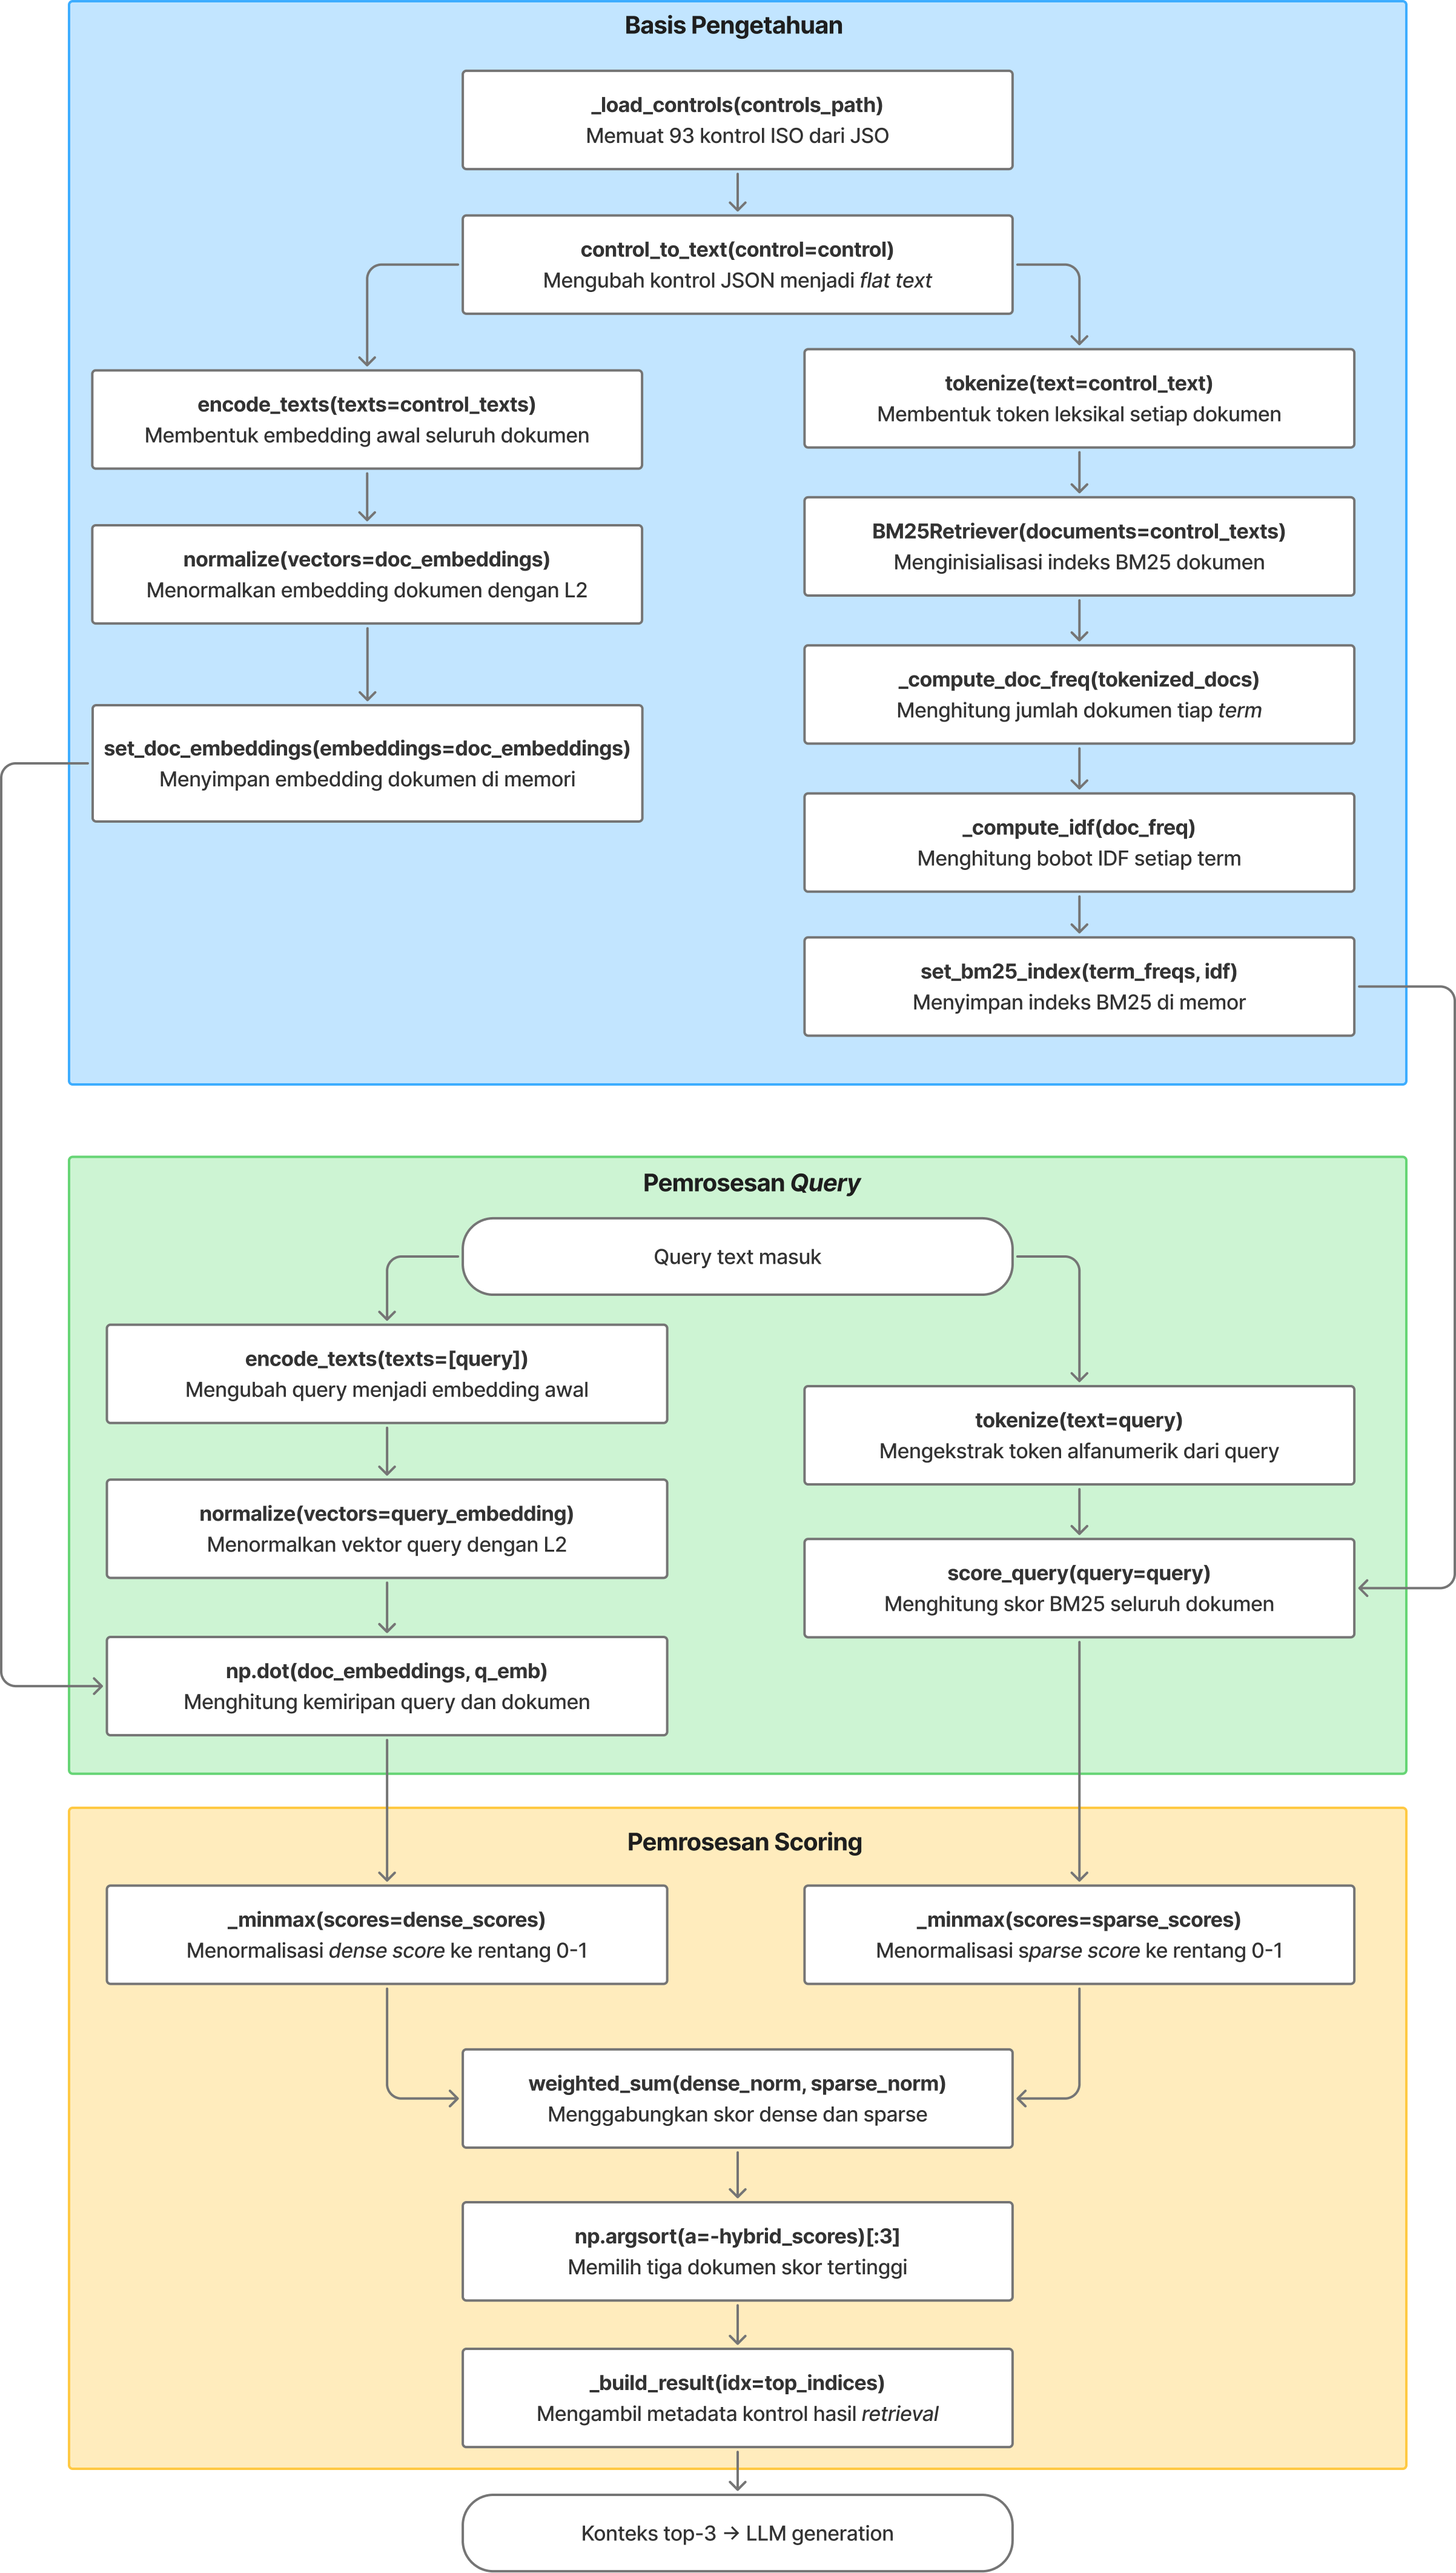
\includegraphics[width=\columnwidth,keepaspectratio]{../Gambar/3.6HybridComponentFinal.png}
\caption{Hybrid retrieval architecture combining BM25 sparse retrieval
with dense embedding retrieval via weighted score fusion.}
\label{fig:hybrid}
\end{figure}

\subsection{Cross-Encoder Reranking and Score Fusion}

The candidate pool from hybrid retrieval is re-evaluated by
BAAI/bge-reranker-v2-m3, a multilingual cross-encoder. The final score
fuses hybrid and cross-encoder scores:
\begin{equation}
  \text{final\_score} = \alpha_r \cdot s_{\text{hybrid}}^{\text{norm}}
  + (1 - \alpha_r) \cdot s_{\text{CE}}^{\text{norm}}
\end{equation}
where $\alpha_r \in \{0.00, 0.25, 0.50, 0.75, 1.00\}$ controls the
hybrid-to-CE ratio. Setting $\alpha_r = 1.0$ reverts to pure hybrid
retrieval; $\alpha_r = 0.0$ uses only cross-encoder scores. Both
$\alpha_d$ and $\alpha_r$ follow the same discrete range and the
complementary weights always sum to 1.

\begin{figure}[H]
\centering
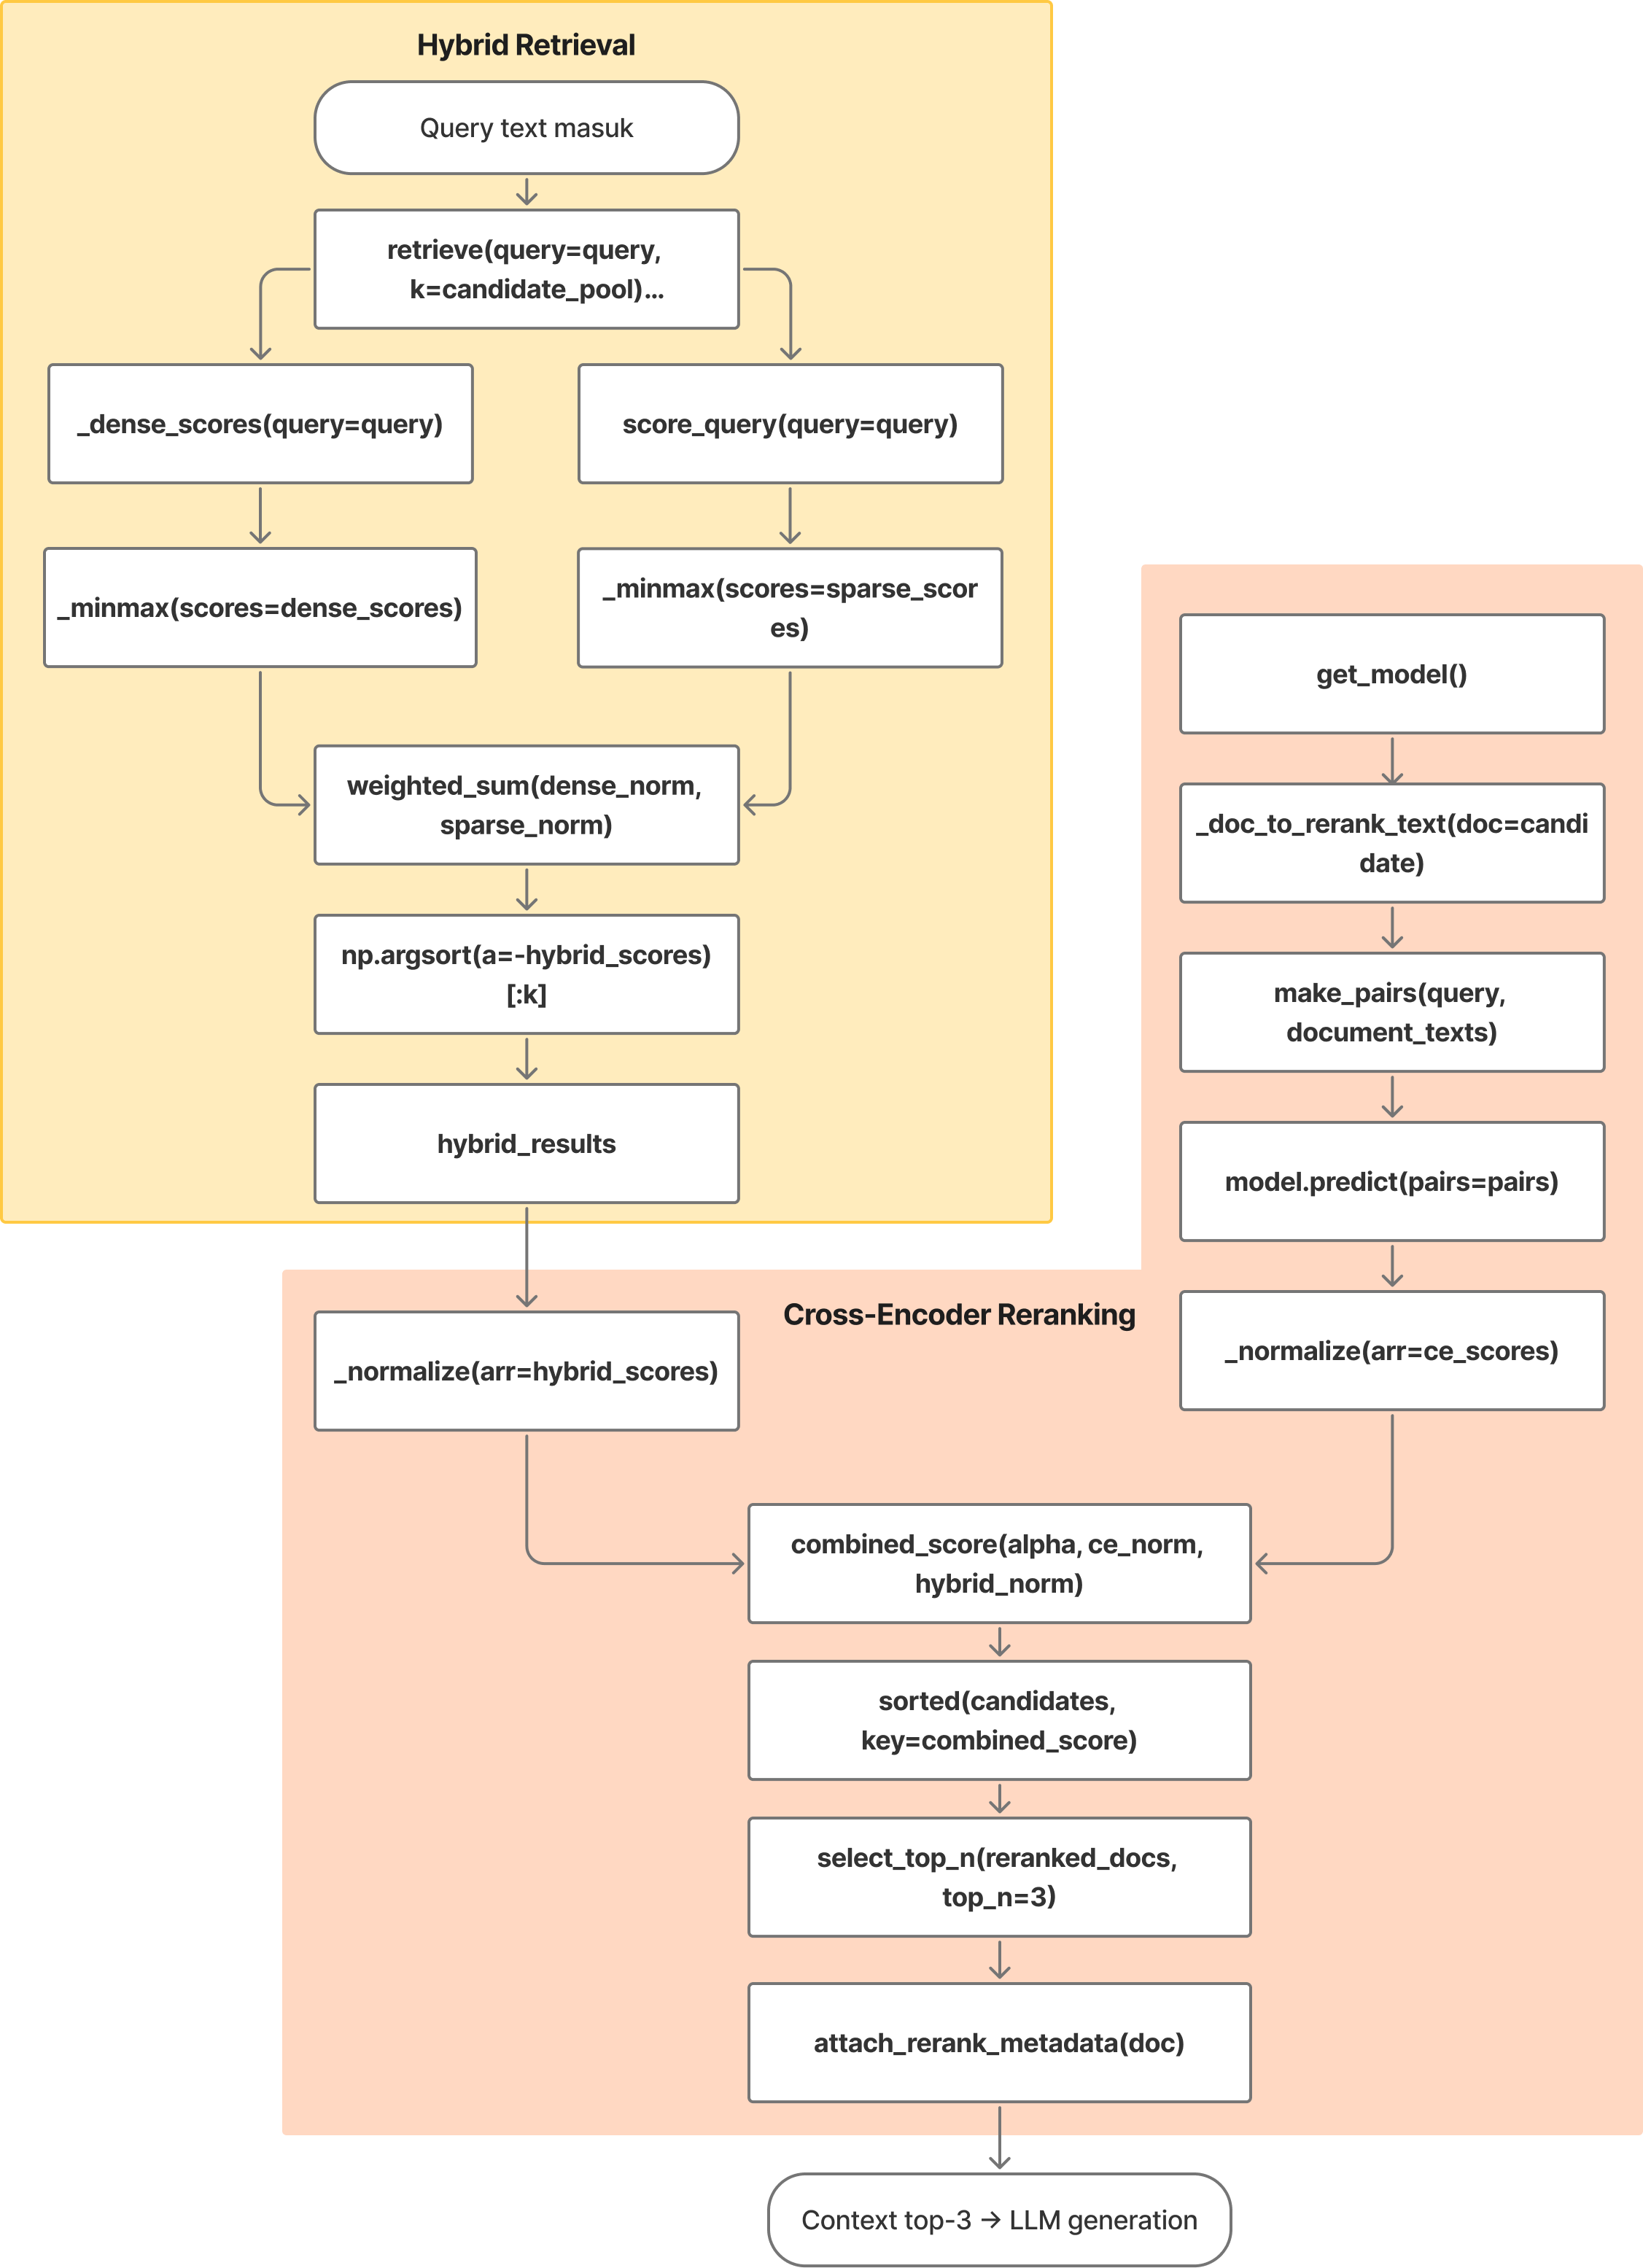
\includegraphics[width=\columnwidth,keepaspectratio]{figs/reranker_component_big.png}
\caption{Cross-encoder reranking pipeline: hybrid retrieval produces a
candidate pool, which the cross-encoder re-evaluates before score fusion.}
\label{fig:reranker}
\end{figure}

\subsection{Experimental Design}

Three sequential experimental scenarios are conducted, where each
subsequent scenario uses the optimal configuration from the previous one:

\textbf{Scenario~1: Dense/Sparse Weight Composition.}
Five configurations are tested: $w_{\text{dense}} \in \{0.00, 0.25, 0.50,
0.75, 1.00\}$.

\textbf{Scenario~2: Candidate Pool Size.}
Four pool sizes are tested: $k \in \{5, 10, 15, 20\}$, using the optimal
dense/sparse composition from Scenario~1.

\textbf{Scenario~3: Score Fusion Weight.}
Five $\alpha$ values are tested: $\alpha \in \{0.00, 0.25, 0.50, 0.75,
1.00\}$, using optimal configurations from Scenarios~1 and~2.

\subsection{Evaluation Metrics and Statistical Testing}

Four metrics are used: Hit@3 and Recall@3 for coverage, and Mean
Average Precision (MAP@3) and NDCG@3 for ranking quality. The Friedman
test~\cite{pereira2015overview} with $\alpha_{\text{sig}} = 0.05$ is
applied to assess statistical significance across configurations, using
77~queries as the blocking factor for repeated-measures comparison.

% ============================================================
\section{Results}
% ============================================================

\subsection{Scenario 1: Dense/Sparse Weight Composition}

\begin{table}[H]
\centering
\caption{Retrieval performance across dense/sparse weight compositions}
\label{tab:hybrid}
\small
\begin{tabular}{lcccc}
\toprule
Dense:Sparse & Hit@3 & Recall@3 & MAP@3 & NDCG@3 \\
\midrule
0.00:1.00 & \textbf{0.961} & 0.485 & 0.407 & 0.525 \\
0.25:0.75 & 0.948 & 0.506 & 0.437 & 0.549 \\
\textbf{0.50:0.50} & 0.935 & \textbf{0.537} & \textbf{0.467} & \textbf{0.575} \\
0.75:0.25 & 0.831 & 0.468 & 0.417 & 0.511 \\
1.00:0.00 & 0.649 & 0.307 & 0.256 & 0.336 \\
\bottomrule
\end{tabular}
\end{table}

\begin{table}[H]
\centering
\caption{Friedman test results for dense/sparse weight compositions}
\label{tab:hybrid_friedman}
\small
\begin{tabular}{lcc}
\toprule
Metric & $\chi^2$ & $p$-value \\
\midrule
Hit@3    & 52.205 & $< 0.000001$ \\
Recall@3 & 53.542 & $< 0.000001$ \\
NDCG@3   & 46.395 & $< 0.000001$ \\
MAP@3    & 46.395 & $< 0.000001$ \\
\bottomrule
\end{tabular}
\end{table}

Table~\ref{tab:hybrid} reports the hybrid retrieval performance across
five dense/sparse weight compositions on 77~queries. The balanced
configuration ($w_{\text{dense}}=0.50$) achieves the highest Recall@3
(0.537), MAP@3 (0.467), and NDCG@3 (0.575). Pure sparse retrieval
($w_{\text{dense}}=0.00$) yields the highest Hit@3 (0.961) but lower
rank-sensitive metrics (MAP@3\,=\,0.407, NDCG@3\,=\,0.525). Pure dense
retrieval ($w_{\text{dense}}=1.00$) performs worst across all four
metrics, with Hit@3\,=\,0.649, Recall@3\,=\,0.307, MAP@3\,=\,0.256,
and NDCG@3\,=\,0.336. The Friedman test
(Table~\ref{tab:hybrid_friedman}) confirms that the differences across
configurations are statistically significant for all four metrics
($\chi^2 \geq 46.395$, $p < 0.000001$).

\subsection{Scenario 2: Candidate Pool Size}

\begin{table}[H]
\centering
\caption{Reranking performance across candidate pool sizes ($w_{\text{dense}}=0.50$)}
\label{tab:pool}
\small
\begin{tabular}{lcccc}
\toprule
Pool & Hit@3 & Recall@3 & MAP@3 & NDCG@3 \\
\midrule
\textbf{5}  & \textbf{0.857} & \textbf{0.468} & \textbf{0.387} & \textbf{0.485} \\
10 & 0.753 & 0.424 & 0.372 & 0.451 \\
15 & 0.701 & 0.394 & 0.343 & 0.418 \\
20 & 0.688 & 0.377 & 0.328 & 0.405 \\
\bottomrule
\end{tabular}
\end{table}

\begin{table}[H]
\centering
\caption{Friedman test results for candidate pool sizes}
\label{tab:pool_friedman}
\small
\begin{tabular}{lcc}
\toprule
Metric & $\chi^2$ & $p$-value \\
\midrule
Hit@3    & 16.760 & 0.000792 \\
Recall@3 & 14.095 & 0.002779 \\
NDCG@3   & 25.776 & 0.000011 \\
MAP@3    & 25.776 & 0.000011 \\
\bottomrule
\end{tabular}
\end{table}

Using the optimal dense/sparse composition from Scenario~1
($w_{\text{dense}}=0.50$), Table~\ref{tab:pool} reports the reranking
performance across four candidate pool sizes. A clear monotonic decline
is observed across all metrics as pool size increases: pool size~5
achieves the highest scores (Hit@3\,=\,0.857, Recall@3\,=\,0.468,
MAP@3\,=\,0.387, NDCG@3\,=\,0.485), whereas pool size~20 yields the
lowest (Hit@3\,=\,0.688, Recall@3\,=\,0.377, MAP@3\,=\,0.328,
NDCG@3\,=\,0.405). Increasing the pool from~5 to~20 degrades Hit@3
by 0.169 and Recall@3 by~0.091. The Friedman test
(Table~\ref{tab:pool_friedman}) confirms significance for all metrics
($\chi^2 \geq 14.095$, $p \leq 0.003$).

\subsection{Scenario 3: Score Fusion Weight}

\begin{table}[H]
\centering
\caption{Retrieval performance across score fusion compositions (Hybrid:CE, $w_{\text{dense}}=0.50$, $k=5$)}
\label{tab:fusion}
\small
\begin{tabular}{lcccc}
\toprule
Hybrid:CE & Hit@3 & Recall@3 & MAP@3 & NDCG@3 \\
\midrule
\textbf{1.00:0.00} & \textbf{0.935} & 0.537 & 0.467 & 0.575 \\
\textbf{0.75:0.25} & \textbf{0.935} & \textbf{0.541} & \textbf{0.470} & \textbf{0.579} \\
0.50:0.50 & 0.896 & 0.528 & 0.452 & 0.553 \\
0.25:0.75 & 0.883 & 0.502 & 0.418 & 0.519 \\
0.00:1.00 & 0.857 & 0.469 & 0.387 & 0.485 \\
\bottomrule
\end{tabular}
\end{table}

\begin{table}[H]
\centering
\caption{Friedman test results for score fusion compositions}
\label{tab:fusion_friedman}
\small
\begin{tabular}{lcc}
\toprule
Metric & $\chi^2$ & $p$-value \\
\midrule
Hit@3    & 10.462 & $0.033$       \\
Recall@3 & 21.245 & $0.000283$    \\
NDCG@3   & 29.639 & $0.000006$    \\
MAP@3    & 28.952 & $0.000008$    \\
\bottomrule
\end{tabular}
\end{table}

Using the optimal configurations from Scenarios~1 and~2
($w_{\text{dense}}=0.50$, $k=5$), Table~\ref{tab:fusion} presents the
retrieval performance across five score fusion compositions. The
hybrid-dominant configuration (Hybrid:CE\,=\,0.75:0.25) achieves the
highest Recall@3 (0.541), MAP@3 (0.470), and NDCG@3 (0.579), marginally
surpassing pure hybrid retrieval (1.00:0.00) which yields
Recall@3\,=\,0.537, MAP@3\,=\,0.467, and NDCG@3\,=\,0.575.
Performance decreases consistently as cross-encoder weight increases:
pure cross-encoder (0.00:1.00) yields the lowest scores
(Hit@3\,=\,0.857, Recall@3\,=\,0.469, MAP@3\,=\,0.387,
NDCG@3\,=\,0.485). The Friedman test
(Table~\ref{tab:fusion_friedman}) confirms significance for all metrics
($\chi^2 \geq 10.462$, $p \leq 0.033$), with rank-sensitive metrics
showing the strongest effect (NDCG@3: $p = 0.000006$;
MAP@3: $p = 0.000008$).

\subsection{Per-Query Comparison: Hybrid vs.\ Cross-Encoder}

\begin{table}[H]
\centering
\caption{Query distribution by winning component across metrics}
\label{tab:winner}
\small
\begin{tabular}{lccc}
\toprule
Metric & Hybrid Superior & CE Superior & Tied \\
\midrule
Hit@3    & 8 (10.4\%)  & 2 (2.6\%)  & 67 (87.0\%) \\
Recall@3 & 24 (31.2\%) & 8 (10.4\%) & 45 (58.4\%) \\
NDCG@3   & 36 (46.8\%) & 15 (19.5\%) & 26 (33.8\%) \\
MAP@3    & 36 (46.8\%) & 15 (19.5\%) & 26 (33.8\%) \\
\bottomrule
\end{tabular}
\end{table}

Table~\ref{tab:winner} reports the per-query comparison between pure
hybrid retrieval ($\alpha_r=1.0$) and pure cross-encoder reranking
($\alpha_r=0.0$) across 77~queries. For rank-sensitive metrics, hybrid
retrieval outperforms the cross-encoder on 36~queries (46.8\%) for both
NDCG@3 and MAP@3, while the cross-encoder outperforms hybrid retrieval on
15~queries (19.5\%). The remaining 26~queries (33.8\%) are tied. For
coverage metrics, Hit@3 shows the least differentiation with 67~queries
(87.0\%) tied, and Recall@3 shows 24~queries (31.2\%) favoring hybrid
retrieval versus 8~queries (10.4\%) favoring the cross-encoder.

% ============================================================
\section{Discussion}
% ============================================================

The results demonstrate that hybrid retrieval and cross-encoder reranking
exhibit complementary strengths, yet hybrid retrieval remains the dominant
contributor to retrieval accuracy in the ISO~27001 domain.

The balanced dense/sparse composition ($w_{\text{dense}}=0.50$) achieves
the best rank-sensitive performance (Table~\ref{tab:hybrid}), indicating
that ISO~27001 control mapping requires both semantic matching to capture
contextual meaning and lexical matching to recognize domain-specific
terminology. The monotonic decline in reranking accuracy as candidate pool
size increases (Table~\ref{tab:pool}) is counter-intuitive: including
less relevant candidates introduces noise that degrades cross-encoder
ranking quality rather than providing additional recall opportunities.
The hybrid-dominant score fusion (0.75:0.25) marginally surpasses pure
hybrid retrieval (Table~\ref{tab:fusion}), confirming that cross-encoder
scores provide supplementary but not dominant signals for this domain.

Despite the overall dominance of hybrid retrieval, the per-query analysis
(Table~\ref{tab:winner}) reveals that cross-encoder reranking outperforms
hybrid retrieval on 15~queries (19.5\%) for NDCG@3 and MAP@3. This
superiority occurs primarily when key phrases in the query lack direct
lexical matches with ISO control terminology, such as when
organizational policy documents use informal language or
cross-lingual terminology that diverges from the standardized ISO~27001
vocabulary (e.g., ``non-legal software'' vs.\ ``licensed software'' in
A.5.32, or ``Authentication'' vs.\ ``autentikasi''). In such cases, the
cross-encoder's joint encoding of query--document pairs captures contextual
relevance that term-based BM25 matching and independent dense embedding
similarity fail to recognize. This weakness of hybrid retrieval is
particularly evident on contextual and procedural queries that describe
organizational frameworks without explicitly referencing ISO terminology,
where the cross-encoder discovers additional ground truth controls through
deeper semantic understanding. These complementary patterns justify
assigning a small weight (25\%) to the cross-encoder in the optimal
score fusion, as it provides marginal yet consistent improvements on
contextually demanding queries without degrading the strong baseline
established by hybrid retrieval.

% ============================================================
\section{Conclusion}
% ============================================================

This paper systematically evaluates retrieval strategies for RAG-based
ISO/IEC~27001:2022 SoA control mapping across three design axes. The key
findings are:

\begin{enumerate}
\item \textbf{Balanced hybrid retrieval is optimal.}
A dense\,=\,0.50, sparse\,=\,0.50 composition achieves the best
Recall@3 (0.537) and NDCG@3 (0.575), confirming that ISO~27001
control mapping requires both semantic and lexical matching. All
differences are statistically significant ($p < 0.001$, Friedman test).

\item \textbf{Smaller candidate pools outperform larger ones.} A pool
size of~5 yields the highest accuracy and lowest latency (9.01~s), with
monotonic degradation as pool size increases. Larger pools introduce noise
that degrades cross-encoder ranking ($p < 0.003$).

\item \textbf{Hybrid-dominant score fusion is preferred.}
Hybrid:CE\,=\,0.75:0.25 achieves the best overall performance
(Recall@3\,=\,0.541, NDCG@3\,=\,0.579). The cross-encoder contribution
is complementary rather than dominant: hybrid retrieval excels on
terminology-driven queries (46.8\%), while cross-encoders benefit
contextual queries (19.5\%).
\end{enumerate}

\noindent\textbf{Future work} includes: validation on diverse organizational
documents, evaluation of smaller pool sizes ($k < 5$), end-to-end RAG
generation evaluation, finer-grained weight search, post-hoc pairwise
statistical tests, and adaptive retrieval strategies that dynamically
adjust fusion weights based on query characteristics.

% ============================================================
\section*{Acknowledgment}
The authors thank the Directorate of Information Technology, Universitas
Gadjah Mada, for providing the policy documents used in this study.

\bibliographystyle{IEEEtran}
\bibliography{references}

\end{document}
